% !TEX root = ../thesis.tex


\chapter{Results and Evaluation}
% \label{cha:dmd_results}
To test the correction algorithm(s), a pattern with full brightness and a black square in the centre (as seen in \cref{fig:dmd_tests_target}) is used, similar to what the experiment uses to make the box potential (\cref{sec:dmd_experimental_setup}). We want to know how the correction handles aberrations in the dark centre. To do this, different testing patterns are added to the camera image in software instead of shining additional light onto the camera. The general goal is then to make the centre as flat as possible.

At first, a fibre pen was used to simulate a deviation from the target pattern, but not only did its intensity fluctuate strongly, making any feedback-based algorithm impossible, it was also obviously not able to produce different aberration patterns.

All the configurations below are tested with two different telescopes, with pixel-to-pixel magnifications of \num{2.2}:1 and \num{5}:1. This means that one pixel on the camera corresponds to $\num{2.2}\times\num{2.2}$ and $\num{5}\times\num{5}$ pixels on the DMD, respectively.
\vfill
\begin{figure}[hbp]
    \centering
    \begin{subfigure}[t]{0.49\textwidth}
        \centering
        \frame{
\includegraphics[width=0.825\linewidth]{DMD/Results/square-target.png}}
        \caption{Target pattern}
        \label{fig:dmd_tests_target}
    \end{subfigure}
    \begin{subfigure}[t]{0.49\textwidth}
        \centering
        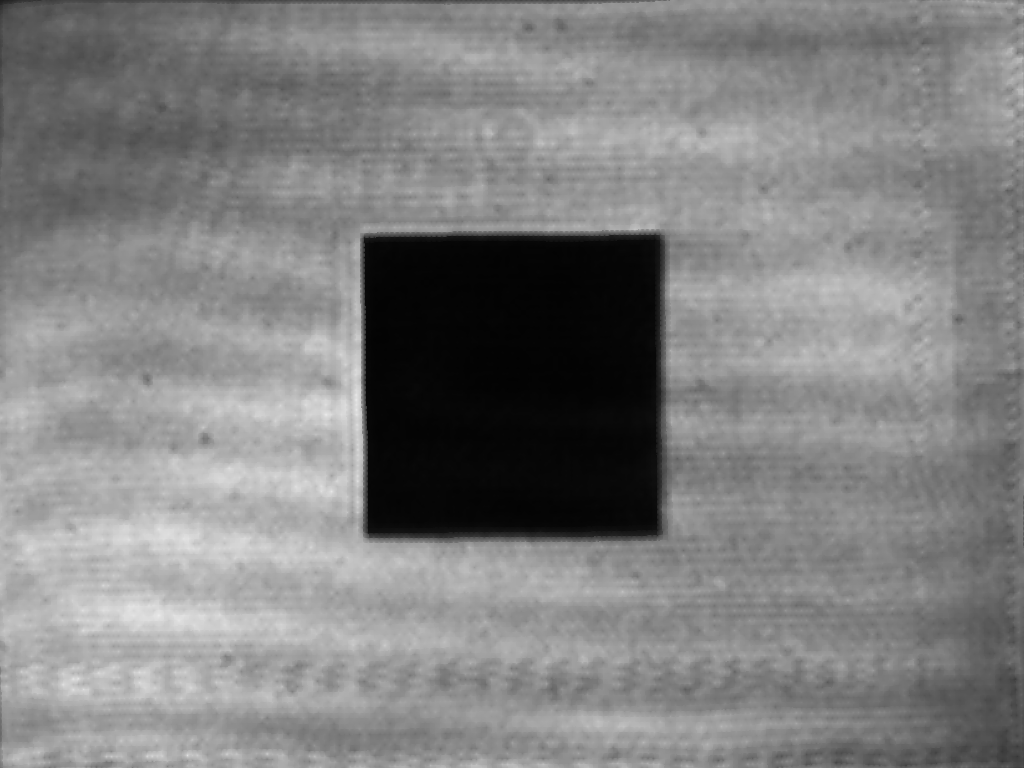
\includegraphics[width=0.825\linewidth]{DMD/Results/ResolutionExamples/15-orig.png}
        \caption{Exemplary camera capture}
    \end{subfigure}
    \caption[Target pattern for the DMD tests]{The centre is a completely dark square with a side length of \SI{300}{px}. (a) shows the target pattern and (b) is an example image taken with the 5:1 magnification telescope.}
\end{figure}


\section{Edge Detection}
\label{sec:results_edgedetection}
We first test the impact of the length scale of the edge detection on the final result. To do this, \emph{no} aberration is added to the image. Instead, we let the algorithm work on the mapped, but unedited camera image.
Because the mapping is not entirely perfect and due to the resolution of the telescope, the bright borders \enquote{leak} into the central dark square which is interpreted as additional, unwanted intensity that needs correction. It is expected that this unwanted correction becomes less drastic with increasing edge detection range.

We vary the edge detection range from $r = \SI{0}{px}$ to $r=\SI{20}{px}$. For each case, we measure the average intensity that is present in the centre after the algorithm has converged. 

In \cref{fig:dmd_results_edgedetection}, we compare this for both magnifications with the maximum intensity that was detected within the portion of the square that has not been excluded by the edge detection. Additionally, \cref{fig:edge_detection_test_example1,fig:edge_detection_test_example2} show two examples of the intensity added by the correction algorithm.
% Additionally, \cref{fig:dmd_results_edgedetection} presents the averaged intensity within the central square of the DMD after the correction for edge detection ranges from \SI{0}{px} to \SI{20}{px}.

It can be seen that that the added intensity indeed decreases with increasing edge detection range and that the corrected intensity follows the maximum detected deviation.

\vfill
% Indeed, by looking at \cref{fig:dmd_results_edgedetection} it is apparent that although low ranges lead to very drastic overcorrections of more than \SI{30}{\percent}, as the detection range is increased, the added intensity decreases. We can also see that the corrected intensity follows the maximum that was detected within the central square. 
%
%
% \begin{figure}[htbp]
%     \centering
%     \begin{subfigure}[t]{0.43\textwidth}
%         \centering
%         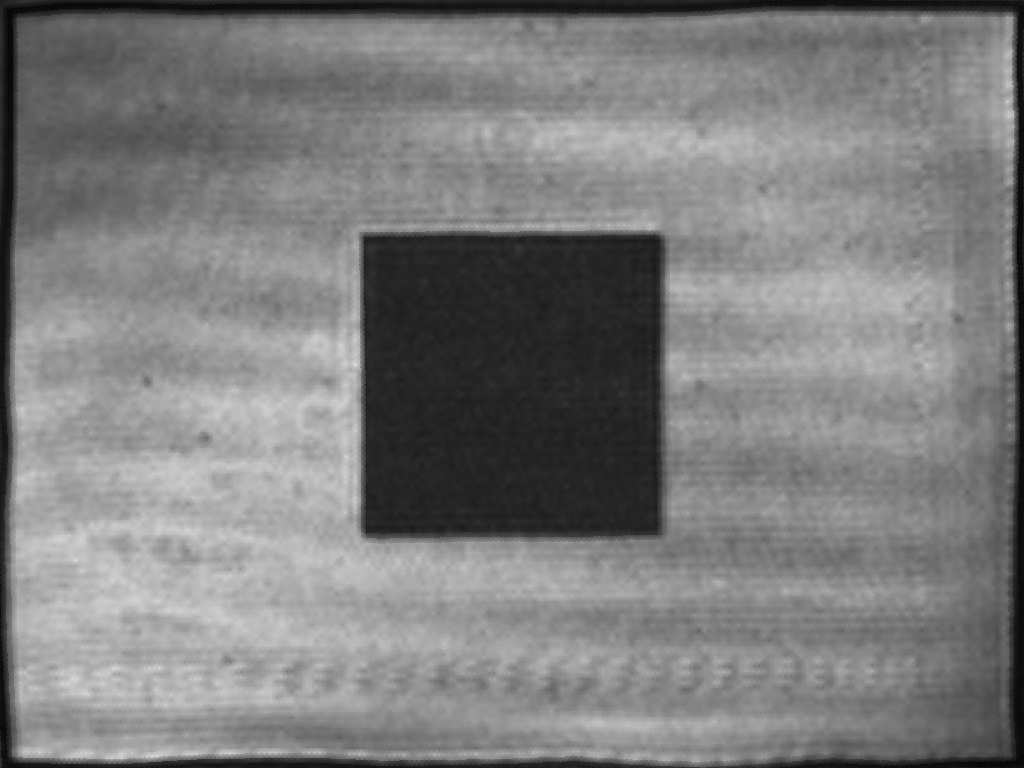
\includegraphics[width=\linewidth]{DMD/Results/EdgeExamples/05}
%         \caption{Detection range: \SI{5}{px}}
%     \end{subfigure}
%     \begin{subfigure}[t]{0.43\textwidth}
%         \centering
%         
\includegraphics[width=\linewidth]{DMD/Results/EdgeExamples/15}
%         \caption{Detection range: \SI{15}{px}}
%     \end{subfigure}
%     \caption[Influence of the edge detection range on the overcorrection of the intensity in the centre]{The contrast in (a) is much lower than in (b).}
%     \label{fig:edge_detection_test_example}
% \end{figure}
% \begin{figure}[hbp]
%     \centering
%     \includegraphics[]{DMD/Results/EdgeDetection}
%     \caption[Test of the edge detection algorithm]{The averaged intensity in the central square ($(300 - 2r)\times (300-2r)$ px) after the correction is shown for both magnifications as well as the maximum intensities detected in this area (black, dotted) and the mean intensity of the original image (grey, dash-dotted).}
%     \label{fig:dmd_results_edgedetection}
% \end{figure}
% \begin{figure}[htbp]
%     \centering
%     % \begin{subfigure}[t]{0.43\textwidth}
%     \begin{subfigure}[t]{0.35\textwidth}
%         \centering
%         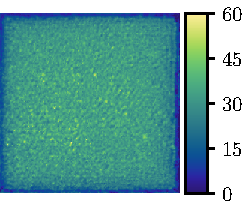
\includegraphics{DMD/EdgeDetectionAddedIntensity05.pdf}
%         \caption{Detection range: \SI{5}{px}}
%     \end{subfigure}
%     \hspace{-0.035\textwidth}
%     % \begin{subfigure}[t]{0.43\textwidth}
%     \begin{subfigure}[t]{0.35\textwidth}
%         \centering
%         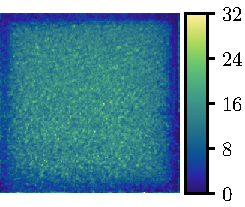
\includegraphics{DMD/EdgeDetectionAddedIntensity15.pdf}
%         \caption{Detection range: \SI{15}{px}}
%     \end{subfigure}
%     \caption[Influence of the edge detection range on the overcorrection of the intensity in the centre]{Both of the examples are taken with the 2.2:1 telescope. Shown is the intensity that was added by the algorithm (corrected $-$ uncorrected).}
%     \label{fig:edge_detection_test_example}
% \end{figure}
\begin{figure}[htbp]
    \centering
    \begin{minipage}[c][8.815cm][t]{0.67\textwidth}
        \vfill
        \centering
        \includegraphics[clip, trim=0 0 0 -6.5px]{DMD/Results/EdgeDetection}
        \subcaption{Intensity in image centre $I$ against the edge detection range $r$}
        \label{fig:dmd_results_edgedetection}
    \end{minipage}
    \hfill
    \begin{minipage}[c][8.815cm][t]{.269\textwidth}
        % \vfill
        \begin{subfigure}[T]{0.72\textwidth}
            \centering
            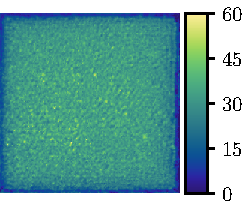
\includegraphics[clip, trim=0 6.5px 31px 0px]{DMD/EdgeDetectionAddedIntensity05.pdf}
            \subcaption{$r=\SI{5}{px}$}
            \label{fig:edge_detection_test_example1}
        \end{subfigure}
        \hspace{-0.06\textwidth}
        \begin{subfigure}[T]{0.24\textwidth}
            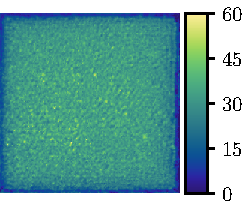
\includegraphics[clip, trim=88.5px -6.5px 0px 0px]{DMD/EdgeDetectionAddedIntensity05.pdf}
        \end{subfigure}
        \vfill
        \begin{subfigure}[T]{0.72\textwidth}
            \centering
            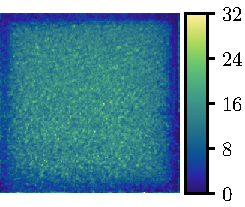
\includegraphics[clip, trim=0 6.5px 31px 0px]{DMD/EdgeDetectionAddedIntensity15.pdf}
            \subcaption{$r=\SI{15}{px}$}
            \label{fig:edge_detection_test_example2}
        \end{subfigure}
        \hspace{-0.06\textwidth}
        \begin{subfigure}[T]{0.24\textwidth}
            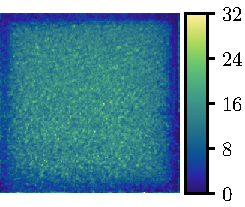
\includegraphics[clip, trim=88.5px -6.5px 0px 0px]{DMD/EdgeDetectionAddedIntensity15.pdf}
        \end{subfigure}
    \end{minipage}
    \caption[Influence of the edge detection range on the intensity in the centre]{(a) shows the mean intensities in the central $(300-2r)\times(300-2r)\,\mathrm{px}$ square of the corrected images for both magnifications along the maximum and mean in the uncorrected ones. (b) and (c) are examples of the difference between the corrected and uncorrected images (2.2:1 magnification). Here, the dark borders show how a part of the edges has been ignored during the correction.}
\end{figure}


\section{Resolution}
\label{sec:dmd_results_resolution}
Next, we want to see how well the algorithm can resolve details. We add artificial deviations that contain sinusoidal wave patterns with varying periods to the camera image:
\begin{equation*}
    I_\text{error} =  A_0 \cdot \frac{1-\cos(2\pi y / \lambda_0)}{2}.
\end{equation*}
Here, $A_0$ is a constant that determines the brightness of the pattern (fixed to a value of 50), $y$ is the vertical coordinate on the image and $\lambda_0$ is the period of the pattern. An example for the case $\lambda_0=\SI{20}{px}$ can be seen in \cref{fig:dmd_wave_error_example}.
% \begin{figure}[bp]
%     \centering
%     \begin{subfigure}[t]{0.24\textwidth}
%         \centering
%         \frame{
\includegraphics[width=\linewidth]{DMD/Results/square-target}}
%         \caption{Target}
%     \end{subfigure}
%     \begin{subfigure}[t]{0.24\textwidth}
%         \centering
%         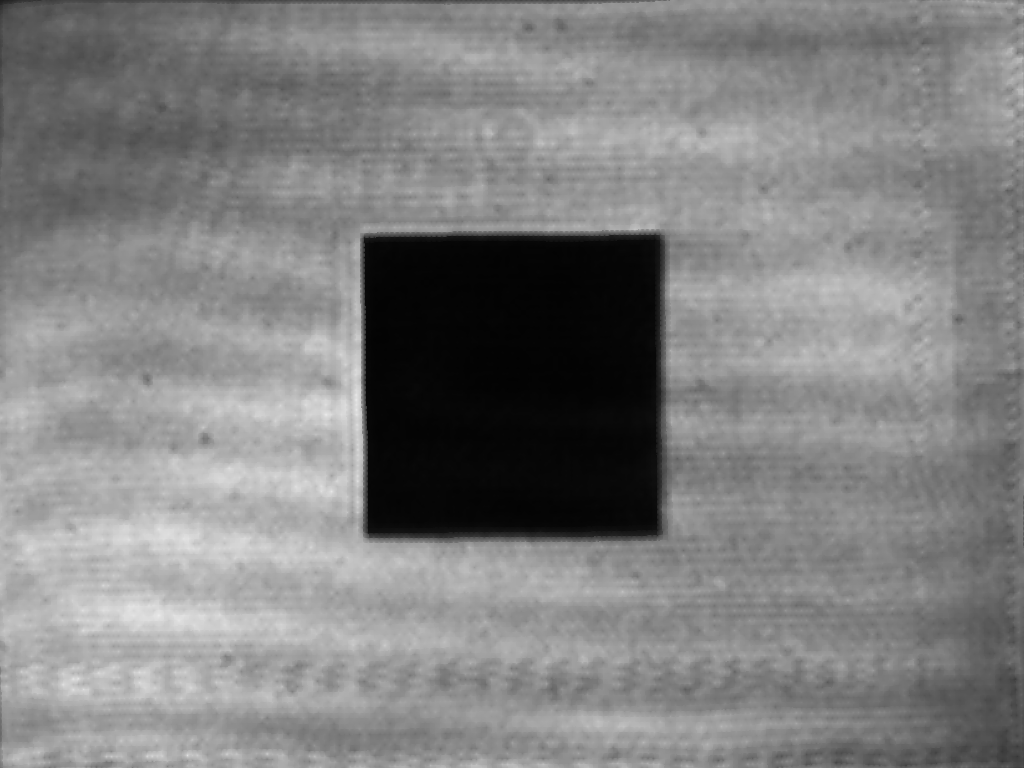
\includegraphics[width=\linewidth]{DMD/Results/ResolutionExamples/15-orig}
%         \caption{Original camera image}
%     \end{subfigure}
%     \begin{subfigure}[t]{0.24\textwidth}
%         \centering
%         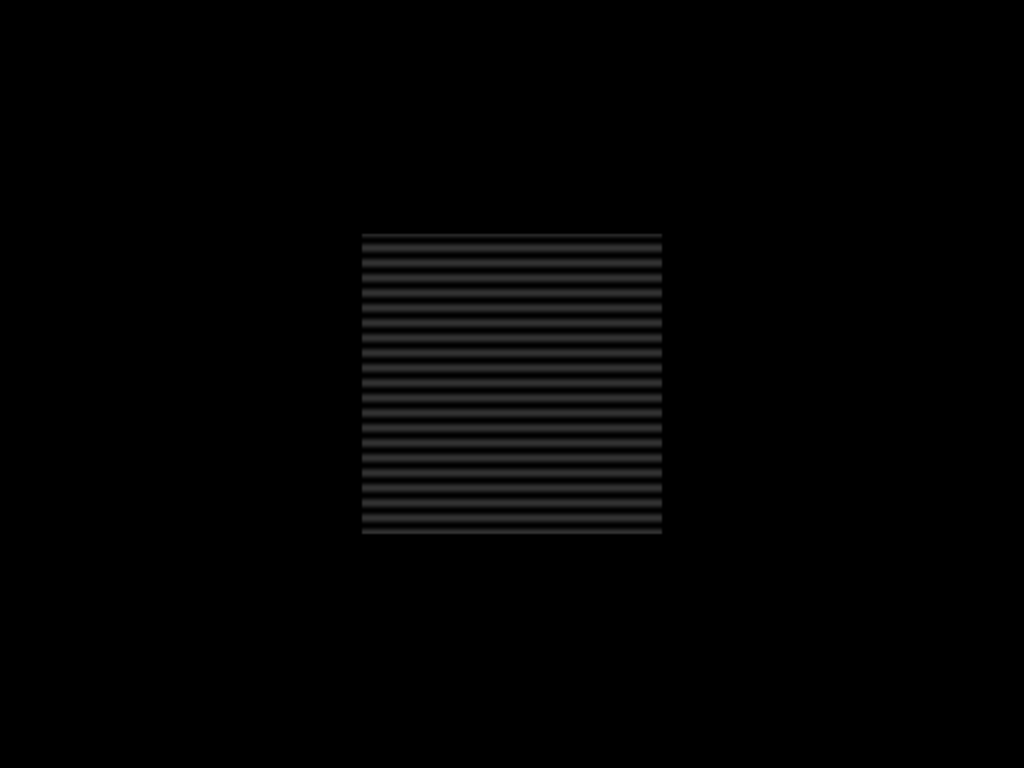
\includegraphics[width=\linewidth]{DMD/Results/ResolutionExamples/15-offs}
%         \caption{Added deviation}
%     \end{subfigure}
%     \begin{subfigure}[t]{0.24\textwidth}
%         \centering
%         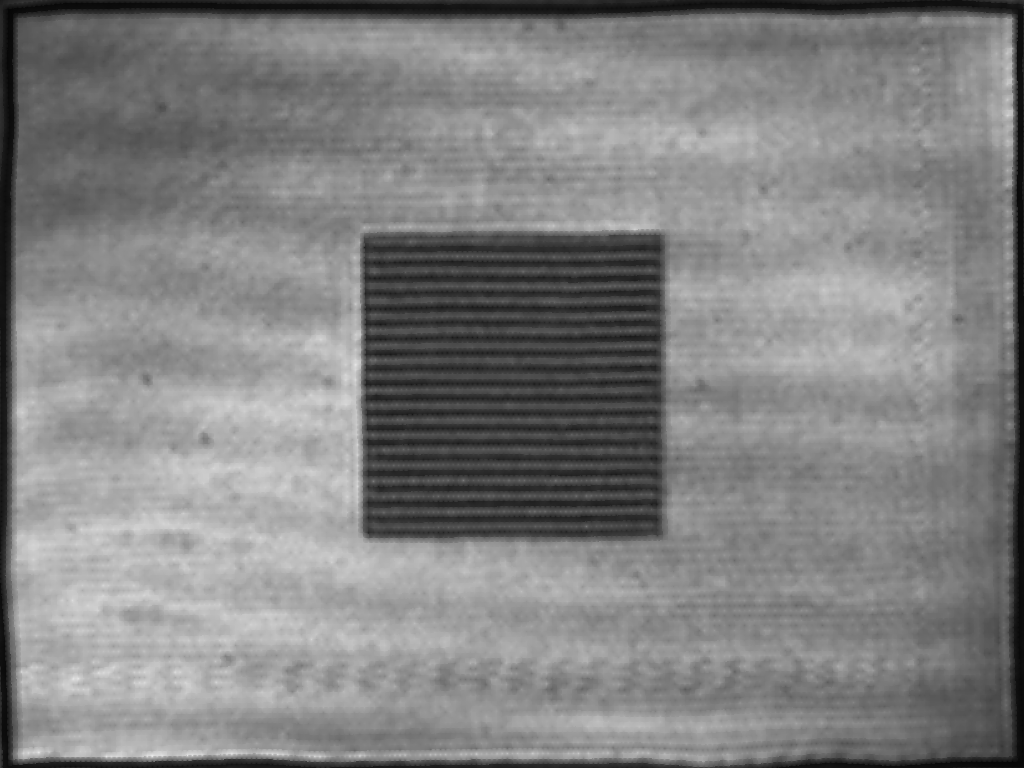
\includegraphics[width=\linewidth]{DMD/Results/ResolutionExamples/15-final}
%         \caption{Corrected image}
%     \end{subfigure}
%     \caption[Test example with added wave pattern]{The pattern seen in (c) appears inverted in the corrected image (d) which can be seen from the shift of the intensity maxima.}
%     \label{fig:dmd_results_resolution_example}
% \end{figure}

After the algorithm has converged, we expect to see the same pattern inverted on the camera image if it was resolved correctly. Then, the pattern can be described by 
\begin{equation} \label{eq:dmd_wave_result}
    I_\text{corr} = C + A \cdot \frac{1 - \cos(2\pi (y-\varphi) / \lambda)}{2}
\end{equation}
with a constant offset $C$ and a phase shift $\varphi$ which is exactly $\pi$ if the pattern was resolved. \Cref{fig:dmd_wave_corr_example} shows this inverted version of the pattern that was generated from \cref{fig:dmd_wave_error_example}.

Lastly, the sum of both intensities should ideally be flat, which is demonstrated in \cref{fig:dmd_wave_sum_example}.

For the analysis, \cref{eq:dmd_wave_result} is fitted to the horizontal average of the central square of the corrected image.
The detected amplitude $A(\lambda_0)$ depending on the period is shown in \cref{fig:dmd_results_resolution_amplitude} and the fits for the different magnifications are displayed in \cref{fig:dmd_results_resolution_cuts,fig:dmd_results_resolution_cuts_old}.

It can be seen that the pattern cannot be resolved for low spacing between the fringes, but after a threshold period $\lambda_\text{threshold}$ is reached, the full amplitude $A_0$ can be reproduced in the corrected image. To determine this threshold, an error function
\begin{equation}
    A(\lambda_0) = \tilde{A}\left[ 1 + \text{erf}\!\left(\frac{\lambda_0 - \lambda_\text{threshold}}{\sigma}\right) \right] \label{eq:errorfunction}
\end{equation}
is fitted to the data. The fit functions are included in \cref{fig:dmd_results_resolution_amplitude} and the resulting coefficients $\tilde{A}$, $\lambda_\text{threshold}$ and $\sigma$ are summarised in \cref{tab:dmd_resolution_fits}. 

If we divide the threshold period by the magnification, we see that $\sim\!\SI{3}{px}$ are necessary on the camera to resolve two lines. This is a great result because with the \SI{1}{px} blur of the camera image taken into account, this is very close to the \enquote{perfect} result of \SI{2}{px}.

% \begin{figure}[htbp]
%     \centering
%     \begin{subfigure}[t]{0.43\textwidth}
%         \centering
%         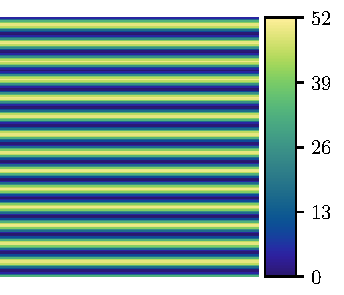
\includegraphics{DMD/Results/ResolutionExamples/20-offs}
%         \caption{Added intensity $I_\text{error}$}
%     \end{subfigure}  
%     \hspace{-.04\textwidth}
%     \begin{subfigure}[t]{0.43\textwidth}
%         \centering
%         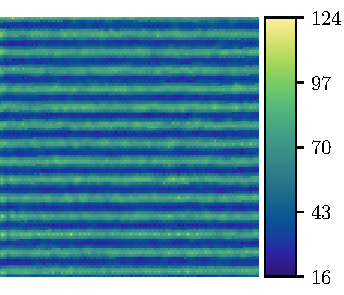
\includegraphics{DMD/Results/ResolutionExamples/20-corr}
%         \caption{Corrected Image}
%     \end{subfigure}
%     % \\[\baselineskip]
%     \begin{subfigure}[t]{0.48\textwidth}
%         \centering
%         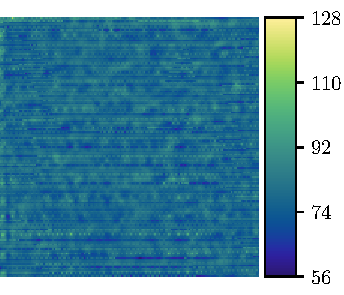
\includegraphics{DMD/Results/ResolutionExamples/20-add}
%         \caption{Sum of (a) and (b)}
%     \end{subfigure}  
%     \caption[Test example with added wave pattern]{Shown is the resolution measurement for $\lambda_0=\SI{20}{px}$ at 5:1 magnification. (a) shows the added intensity pattern, (b) the resulting camera image after the correction has converged and (c) the sum of the previous two images.}
%     \label{fig:dmd_results_resolution_example}   
% \end{figure}
% \vfill
% \begin{figure}[htbp]
%     \centering
%     \begin{subfigure}[t]{0.32\textwidth}
%         \centering
%         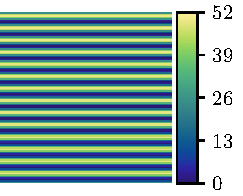
\includegraphics{DMD/Results/ResolutionExamples/20-offs-smaller}
%         \caption{Added intensity $I_\text{error}$}
%     \end{subfigure}  
%     \begin{subfigure}[t]{0.32\textwidth}
%         \centering
%         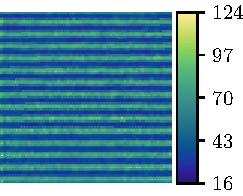
\includegraphics{DMD/Results/ResolutionExamples/20-corr-smaller}
%         \caption{Corrected Image}
%     \end{subfigure}
%     \begin{subfigure}[t]{0.32\textwidth}
%         \centering
%         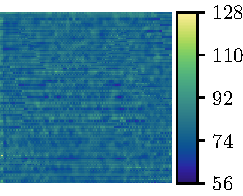
\includegraphics{DMD/Results/ResolutionExamples/20-add-smaller}
%         \caption{Sum of (a) and (b)}
%     \end{subfigure}  
%     \caption[Test example with added wave pattern]{Shown is the resolution measurement for $\lambda_0=\SI{20}{px}$ at 5:1 magnification. (a) shows the added intensity pattern, (b) the resulting camera image after the correction has converged and (c) the sum of the previous two images.}
%     \label{fig:dmd_results_resolution_example}   
% \end{figure}
\begin{figure}[htbp]
    \centering
    \begin{subfigure}[T]{0.24\textwidth}
        \centering
        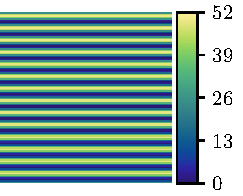
\includegraphics[clip, trim=0 5.6px 34px 0px]{DMD/Results/ResolutionExamples/20-offs-smaller}
        \caption{$I_\text{error}$}
        \label{fig:dmd_wave_error_example}
    \end{subfigure}
    \hspace{-1.7em}
    \begin{subfigure}[T]{0.075\textwidth}
        \centering
        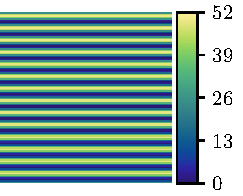
\includegraphics[clip, trim=83px 0px 0px 0px]{DMD/Results/ResolutionExamples/20-offs-smaller}
    \end{subfigure}
    \hfill
    \begin{subfigure}[T]{0.24\textwidth}
        \centering
        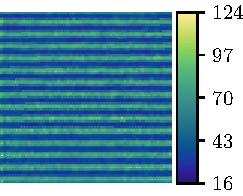
\includegraphics[clip, trim=0 5.6px 34px 0px]{DMD/Results/ResolutionExamples/20-corr-smaller}
        \caption{$I_\text{corr}$}
        \label{fig:dmd_wave_corr_example}
    \end{subfigure}
    \hspace{-1.7em}
    \begin{subfigure}[T]{0.075\textwidth}
        \centering
        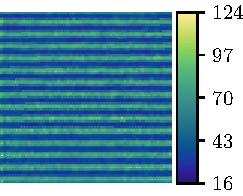
\includegraphics[clip, trim=83px 0px 0px 0px]{DMD/Results/ResolutionExamples/20-corr-smaller}
    \end{subfigure}
    \hfill
    \begin{subfigure}[T]{0.24\textwidth}
        \centering
        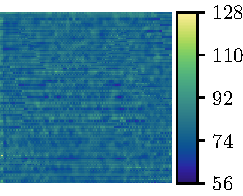
\includegraphics[clip, trim=0 5.6px 34px 0px]{DMD/Results/ResolutionExamples/20-add-smaller}
        \caption{$I_\text{error} + I_\text{corr}$}
        \label{fig:dmd_wave_sum_example}
    \end{subfigure}
    \hspace{-1.7em}
    \begin{subfigure}[T]{0.075\textwidth}
        \centering
        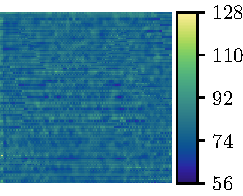
\includegraphics[clip, trim=83px 0px 0px 0px]{DMD/Results/ResolutionExamples/20-add-smaller}
    \end{subfigure}  
    \caption[Test example with added wave pattern]{Shown is the resolution measurement for $\lambda_0=\SI{20}{px}$ at 5:1 magnification. (a) shows the added intensity pattern, (b) the resulting camera image after the correction has converged and (c) the sum of the previous two images.}
    \label{fig:dmd_results_resolution_example}   
\end{figure}
% \vfill
\begin{figure}[htbp]
    \centering
    \includegraphics[]{DMD/Results/LengthScaleAmp}
    \caption[Detected amplitude of the wave pattern depending on the period]{The solid lines are error function fits (\cref{eq:errorfunction}, results in \cref{tab:dmd_resolution_fits}). Except for the first datapoint of the lower magnification, the errorbars are too small to be visible. The dotted green line is a continuation of the fitted function for this magnification over the rest of the data range.}
    \label{fig:dmd_results_resolution_amplitude}
\end{figure}

\begin{table}[htbp]
    \centering
    \caption[Results of the fits in \cref{fig:dmd_results_resolution_amplitude}]{The parameters $\tilde{A}$, $\lambda_\text{threshold}$ and $\sigma$ are defined by \cref{eq:errorfunction}.}
    \begin{tabular}{cS[table-format=2.2(2)]S[table-format=2.2(2)]S[table-format=1.2(2)]}
        \toprule
        \multicolumn{1}{c}{Magnification} & \multicolumn{1}{c}{$\tilde{A}$} & \multicolumn{1}{c}{$\lambda_\text{threshold}$/px} & \multicolumn{1}{c}{$\sigma$/px} \\
        \midrule
        2.2:1 & 53.11+-0.64 & 6.71+-0.18 & 1.07+-0.21 \\
        \phantom{2.2}\negphantom{5}5:1   & 50.37+-0.22 & 13.49+-0.08 & 2.48+-0.15 \\
        \bottomrule
    \end{tabular}
    \label{tab:dmd_resolution_fits}
\end{table}


\section{Error Distribution Analysis}
We can now combine the images from the tests in \cref{sec:results_edgedetection,sec:dmd_results_resolution} and analyse the frequency with which errors of different intensities occur in the corrected images. For the edge detection images, the errors are calculated as the difference of the pixel intensity from the mean across the central square, excluding the respective edge area. From the resolution test, the sum of the deviation and the corrected images are evaluated, but only where the deviation was fully resolved ($\lambda \geq \SI{9}{px}$ and $\lambda \geq \SI{19}{px}$ for the 2.2:1 and 5:1 magnification, respectively).

\Cref{fig:dmd_error_histogram} shows a histogram of the different errors that occur. Although, the RMS error is very low for both magnifications, much larger deviations from occur as well. However, large deviations are very uncommon. 
To quantify this, we show a few important error quantiles in \cref{tab:dmd_error_quantiles}. 
These demonstrate that the corrected images have a very small amount of noise overall. Only very few pixels exhibit large deviations.
% To quantify this, we measure how large the error $\tilde{\Delta}$ is, such that an amount $C$ of pixels has (absolute) errors less than $\tilde{\Delta}$, where $C\in \{\SI{90}{\percent},\SI{95}{\percent},\SI{99}{\percent},\SI{99.9}{\percent}\}$. These are summarised in \cref{tab:dmd_error_quantiles}.
\begin{figure}[htbp]
    \centering
    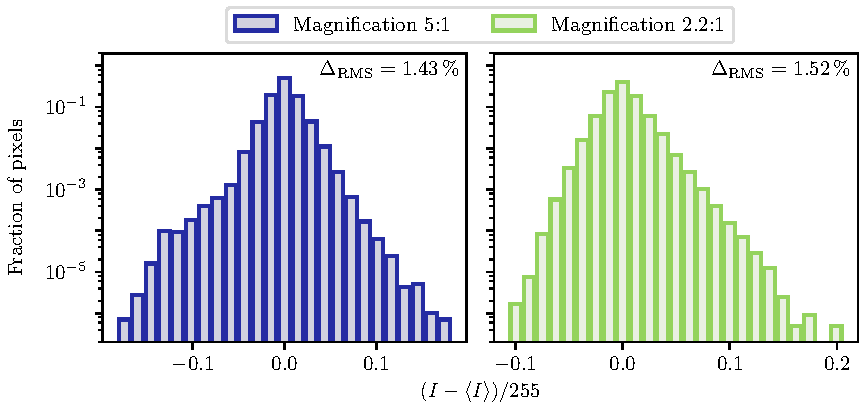
\includegraphics{DMD/Results/ErrorAnalysis}
    \caption[Logarithmic histogram of the single pixel intensity errors]{The data represents the difference from the mean for all the flat images from \cref{sec:results_edgedetection,sec:dmd_results_resolution}.}
    \label{fig:dmd_error_histogram}
\end{figure}
\begin{table}[htbp]
    \centering
    \caption[Error quantiles for the corrected images]{$\tilde{\Delta}$ is the error from the mean such that the deviation of an amount $C$ of pixels is less than $\tilde{\Delta}$.}
    \label{tab:dmd_error_quantiles}
    \begin{tabular}{S[table-format=2.1]S[table-format=1.2]S[table-format=1.2]}
        \toprule
        \multicolumn{1}{c}{$C/\si{\percent}$} & \multicolumn{2}{c}{$\tilde{\Delta}/\si{\percent}$} \\
        \cmidrule{2-3}
            & \multicolumn{1}{c}{Magnification 2.2:1} & \multicolumn{1}{c}{Magnification 5:1} \\
        \midrule
        90 & 2.41 & 2.27 \\
        95 & 3.15 & 2.99 \\
        99 & 4.86 & 4.58 \\
        99.9 & 7.61 & 8.12 \\
        \bottomrule
    \end{tabular}
\end{table}


\section{Randomised Noise Floor}
The last test is to add a random noise pattern with different levels of imhomogeneity as a deviation to the camera image. After the algorithm has converged, this noise pattern should appear as a negative in the camera image. We then add the same noise pattern back on top, which would yield an image with no remaining deviation in case the algorithm works perfectly. Thus, evaluating the remaining RMS error (over the central $300\times \SI{300}{px}$ square) is a measure of the correction quality. 

We have already established in the previous step that the patches need to have a certain separation to be resolvable. It is therefore not as straightforward as using a noisy image with individual randomised pixel intensities. In this test, we create noise of a certain but arbitrary height $H$ (pixel brightness value on a scale from 0 to 255) by distributing random values from a Gaussian distribution with mean $H$ and standard deviation $H$ over a rectangle with half the side lengths of the DMD. The choice of a Gaussian distribution is arbitrary. Intensities lower than 0 are cut off. The complete pattern is then blurred using a Gaussian filter with a radius of \SI{7}{px} and scaled up to the full size of the DMD. This ensures that the noise pattern can be resolved by the correction algorithm. An example of a noise pattern generated this way is shown in \cref{fig:dmd_noise_example}.
% \begin{figure}[bp]
%     \centering
%     % 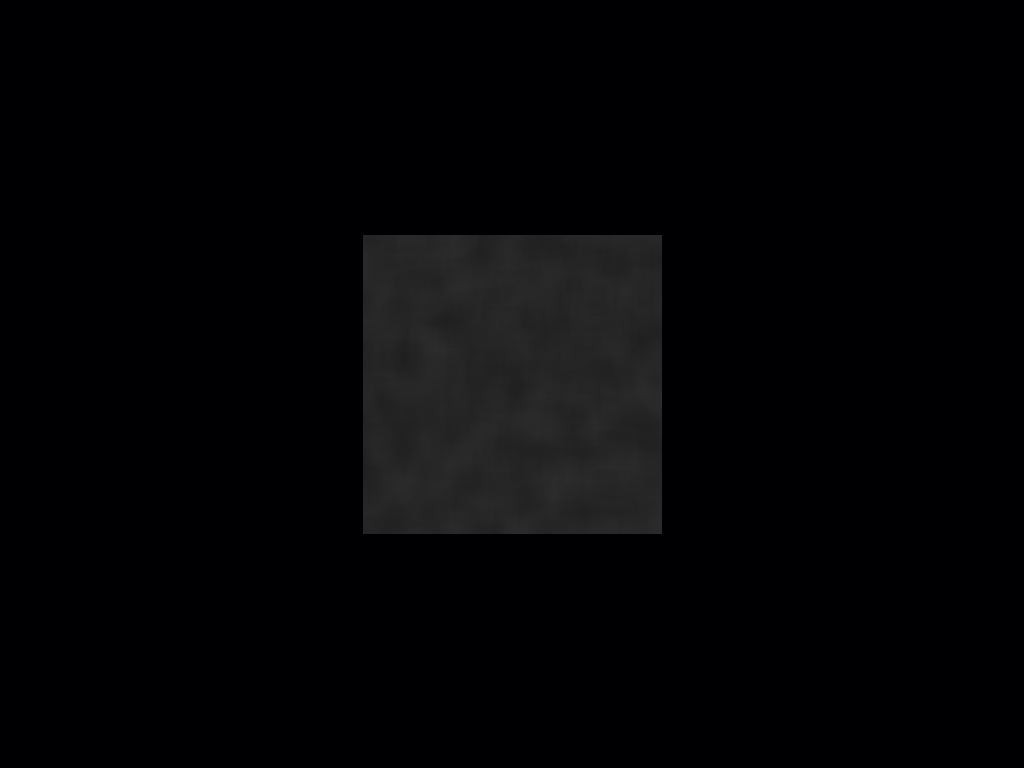
\includegraphics[width=.43\textwidth]{DMD/Results/NoiseExamples/35}
%     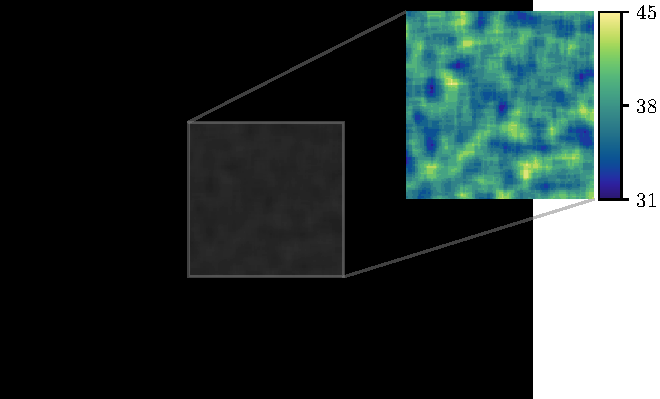
\includegraphics{DMD/noiseExample}
%     \caption[Artificial noise floor pattern]{The pattern shown here was generated with a setting of $H=35$. The inset shows the central $300\times \SI{300}{px}$ square in a false colour scale to make the noise more visible.}
%     \label{fig:dmd_noise_example}
% \end{figure}

To get statistically significant results, we run the test 100 times for each height $H$ and each magnification.
%
% \Cref{tab:dmd_noise_results} shows the averages for the initial RMS error of the noise pattern $\Delta_0$, the final RMS error after convergence is reached $\Delta_\text{final}$ and the necessary number of iterations $N$. 
\Cref{tab:dmd_noise_results} summarises the test results and \cref{fig:dmd_results_noise_evolution} shows the evolution of the RMS error after each iteration of the correction algorithm.

In all cases, the final RMS error is below \SI{1}{\percent} and in most cases, less than 12 iterations were necessary to reach this value. With increasing noise floor height, a larger portion of the DMD's dynamic range can be utilised for the correction, giving a larger improvement relative to the initial error. 

\vfill
\begin{figure}[hbp]
    \centering
    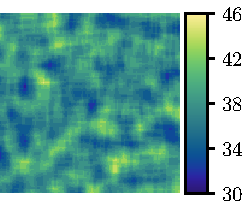
\includegraphics{DMD/height35}
    \caption[Artificial noise floor pattern]{The pattern shown here was created with a setting of $H=35$. Note that -- due to the way in which these randomised patterns are generated -- the mean and standard deviation of the final pattern do not equal the initial value for $H$.}
    \label{fig:dmd_noise_example}
\end{figure}
\vfill

\begin{table}[bp]
    \centering
    \caption[Summarised results from the noise pattern corrections]{$H$ is the height of the noise pattern given in pixel brightness (0 to 255), $\Delta_0$ the initial RMS error caused by the added pattern, $\Delta_\text{final}$ the average of the achieved RMS error after correction and $N$ the average number of iterations necessary until the correction converged.}
    \begin{tabular}{cS[table-format=2]S[table-format=2.2(1)]S[table-format=2.2(1)]S[table-format=2.1(2),separate-uncertainty=true]}
        \toprule
        \multicolumn{1}{c}{Magnification} & \multicolumn{1}{c}{$H$} & \multicolumn{1}{c}{$\Delta_0$/\si{\percent}} & \multicolumn{1}{c}{$\Delta_\text{final}$/\si{\percent}} & \multicolumn{1}{c}{$N$} \\
        \midrule
        {\multirow{4}{*}{\num{2.2}:1}} & 5 & 2.07 +- 0.01 & 0.68 +- 0.03 & 8.3 +- 0.9 \\
        & 15 & 6.28 +- 0.03 & 0.74 +- 0.03 & 8.8 +- 1.2 \\
        & 25 & 10.48 +- 0.06 & 0.78 +- 0.03 & 8.6 +- 1.1 \\
        & 35 & 14.68 +- 0.09 & 0.88 +- 0.04 & 8.2 +- 1.2 \\
        \midrule
        {\multirow{4}{*}{\negphantom{5}\phantom{\num{2.2}}5:1}} & 5 & 2.07 +- 0.01 & 0.56 +- 0.03 & 9.9 +- 1 \\
        & 15 & 6.28 +- 0.03 & 0.64 +- 0.04 & 9.1 +- 0.9 \\
        & 25 & 10.48 +- 0.06 & 0.75 +- 0.05 & 8.5 +- 1.3 \\
        & 35 & 14.68 +- 0.09 & 0.82 +- 0.05 & 9.2 +- 1.4 \\
        \bottomrule
    \end{tabular}
    \label{tab:dmd_noise_results}
\end{table}

% Finally, we show the evolution of the deviation relative to $\Delta_0$ over the first $\tilde{N} = \mu_N + \sigma_N$ iterations (average $+$ one standard deviation, see \cref{tab:dmd_noise_results}) in \cref{fig:dmd_results_noise_evolution}. The reason that the relative error starts above $1$ in some cases is that the edge detection range was not high enough, meaning that the maximum deviation detected at the edges of the square was higher than from the noise pattern.
\begin{figure}[bp]
    \centering
    \includegraphics[]{DMD/Results/IterationsErrorEvo}
    \caption[Error evolution in the correction of a randomised noise pattern]{In some of the graphs, the relative error is larger than 1 in the first iterations, because the edge detection range was too small and the detected error was larger than the added deviation. The number of iterations shown in the individual graphs corresponds to $N + \sigma_N$, where $\sigma$ is the standard uncertainty, with the values from \cref{tab:dmd_noise_results}. Errorbars are omitted because they are too small to be visible. }
    \label{fig:dmd_results_noise_evolution}
\end{figure}


% This is an excellent result and strongly indicates that this method can indeed be used to correct for additional light that does not come from the DMD itself.

% \begin{figure}[htbp]
%     \centering
%     \includegraphics[]{DMD/Results/IterationsFinalError}
%     \caption{COOL CAPTION GOES HERE}
%     \label{fig:dmd_results_noise_finalerror}
% \end{figure}
% \begin{figure}[htbp]
%     \centering
%     \includegraphics[]{DMD/Results/IterationsNumber}
%     \caption{COOL CAPTION GOES HERE}
%     \label{fig:dmd_results_noise_number}
% \end{figure}
